\section{Proximity-Based Approaches}


\begin{frame}{Proximity-Based Approaches}
	\begin{itemize}
		\item \textbf{Assumption:} Outliers are far away
		\item Quantifies how far away objects are from each other by employing a distance measure
		\item Two types of proximity-based outlier detection methods:
	\end{itemize}

	\begin{columns}
		\begin{column}{0.55\textwidth}
			\begin{center}
				\textbf{Distance-Based Methods}
			\end{center}
			\begin{itemize}
				\item Consults the neigbhorhood.
				\item Neighborhood defined by a given radius.
				\item Objects are considered as outlier if its neigbhorhood does not contain enough objects.
				\item Different methods: distance-based with nested loop, grid-based.
			\end{itemize}
		\end{column}

		\begin{column}{0.45\textwidth}
			\begin{center}
				\textbf{Density-Based Methods}
			\end{center}
			\begin{itemize}
				\item Investigates the density of an object and that of its neigbors.
				\item Object is consideres an outlier if density is lower than that of its neigbors.
			\end{itemize}
		\end{column}
	\end{columns}
\end{frame}


\begin{frame}{Distance-Based Outlier Detection: Method with a Nested Loop I}
	\begin{itemize}
		\item Suppose we have:
		      \begin{itemize}
			      \item a set of data objects $D$ with $n$ objects, and
			      \item a user-specified threshold $r$ with $r > 0$
		      \end{itemize}
		\item For each object $\mathbf{o}\in D$ examine the number of other objects in the $r$-neighborhood of $\mathbf{o}$.
		\item If most objects in $D$ are far away from $\mathbf{o}$, then $\mathbf{o}$ is an outlier.
		\item Formally: \textbf{An object $\mathbf{o}$ is a \underline{$\mathbf{DB}(r, \pi)$-outlier}, iff}
		      \begin{align*}\label{db-outlier}
			      \frac{||\{\mathbf{o'} \; \vert \; d(\mathbf{o},\mathbf{o'}) \leq r \}|| }{||D||} \leq \pi.
		      \end{align*}

		      where
		      \begin{itemize}
			      \item $d(\mathbf{o},\mathbf{o}')$ is a distance function of two objects $\mathbf{o}$ and $\mathbf{o}'$
			      \item $\pi$ with $0\leq\pi\leq1$ is a fraction threshold.
		      \end{itemize}
		\item Determine if an object $\mathbf{o}$ is an outlier by taking a look at the $k$-nearest neighbor $\mathbf{o}_k$ where $k=\ceil*{\pi n}$
		\item $\mathbf{o}$ is an outlier, if $d(\mathbf{o}, \mathbf{o}_k) > r$.
	\end{itemize}
\end{frame}


\begin{frame}{Distance-Based Outlier Detection: Method with a Nested Loop II}
	\begin{columns}[t]
		\begin{column}{0.5\textwidth}
			\vspace*{-0.5em}
			\textbf{Efficient computation: {\color{airforceblue}Nested-loop algorithm}:}
			\begin{itemize}
				\item For every object $\mathbf{o}_i\in D$ calculate distance with every other object $\mathbf{o}_j \in D$ where $i\neq j$.
				\item Also count the number of objects in the $r$-neighborhood of $\mathbf{o}_i$.
				\item Terminate inner loop if $\pi n$ objects found in distance $r$: $\mathbf{o}_i$ is no $\mathbf{DB}(r, \pi)$-outlier.
				\item Otherwise do not terminate: $\mathbf{o}_i$ is an outlier.
			\end{itemize}
			\textbf{Efficiency:}
			\begin{itemize}
				\item $\mathcal{O}(n^2)$, but linear CPU-time w.r.t. data set size.
				\item Early termination: small dataset with few outliers.
				\item Costly for large dataset not fitting into RAM.
			\end{itemize}
		\end{column}

		\begin{column}{0.5\textwidth}
			\vspace*{1em}
			\scriptsize
			\begin{algorithm}[H]
				\SetAlgoVlined
				\KwData{a set of objects $D=\{\mathbf{o}_1, \dots, \mathbf{o}_n\}$, threshold $r$, fraction threshold $\pi$}
				\KwResult{$\mathbf{DB}(r, \pi)$-outlier in $D$}
				\BlankLine
				\ForEach{$\mathbf{o}_i\in D$}{
					\texttt{count} $\leftarrow 0$\;
					\ForEach{$\mathbf{o}_j\in D$}{
						\If{$\mathbf{o}_i \neq \mathbf{o}_j$ and $d(\mathbf{o}_i, \mathbf{o}_j)\leq r$}{
							\texttt{count} $\leftarrow$ \texttt{count} $+ 1$\;
							\If{\texttt{count}$\geq \pi n$}{
								\tcc{$\mathbf{o}_i$ cannot be a $\mathbf{DB}(r, \pi)$-outlier}
								exit inner loop\;
							}
						}
					}
				}
				\BlankLine
				\KwRet{
					set of all $\mathbf{DB}(r, \pi)$-outlier in $D$
				}
			\end{algorithm}
		\end{column}
	\end{columns}
\end{frame}


\begin{frame}{Distance-Based Outlier Detection: Method with a Nested Loop III}\textbf{Why is efficiency still a concern?}
	\begin{itemize}
		\item If the complete set of objects cannot be held in main memory, \\
		      there is significant cost for I/O swapping.
	\end{itemize}
	\textbf{The major cost:}
	\begin{enumerate}
		\item \textcolor{faugray}{\textbf{All-Pair-Similarity:}}

		      Each object is tested against the whole data set, \\
		      why not only against its close neighbors?
		\item \textcolor{faugray}{\textbf{Iterative Approach:}}

		      Objects are checked one by one, why not group by group?
	\end{enumerate}

	Improvements can be handled by using a \underline{grid-based method}.
\end{frame}


\begin{frame}{Distance-Based Outlier Detection: A Grid-Based Method I}
	\begin{itemize}
		\item \textbf{CELL:}
		      \begin{itemize}
			      \item Data space is partitioned into a multi-dimensional grid.
			      \item Each cell is a hyper cube with diagonal length $\frac{r}{2}$.
			            \begin{itemize}
				            \item $r$-distance threshold parameter.
				            \item $l$-dimensions: edge of each cell $r / (2\sqrt{l})$ long.
			            \end{itemize}
		      \end{itemize}
		\item \textbf{Level-1 cells:}
		      \begin{itemize}
			      \item Immediately next to cell $\mathbf{C}$.
			      \item For any possible point $\mathbf{x}$ in $\mathbf{C}$ and \\
			            any possible point $\mathbf{y}$ in a level-1 cell: $d(x,y) \leq r$.
		      \end{itemize}
		\item \textbf{Level-2 cells:}
		      \begin{itemize}
			      \item One or two cells away from $\mathbf{C}$.
			      \item For any possible point $\mathbf{x}$ in cell $\mathbf{C}$ and \\
			            any point $\mathbf{y}$ such that $d(x,y) \geq r$, $\mathbf{y}$ is in a level-2 cell.
		      \end{itemize}
		\item Example: Given a 2-dimensional data set, the length of each cell edge is $\frac{r}{2\sqrt{2}}$.
	\end{itemize}
	\tikzoverlay at (10cm,6cm) {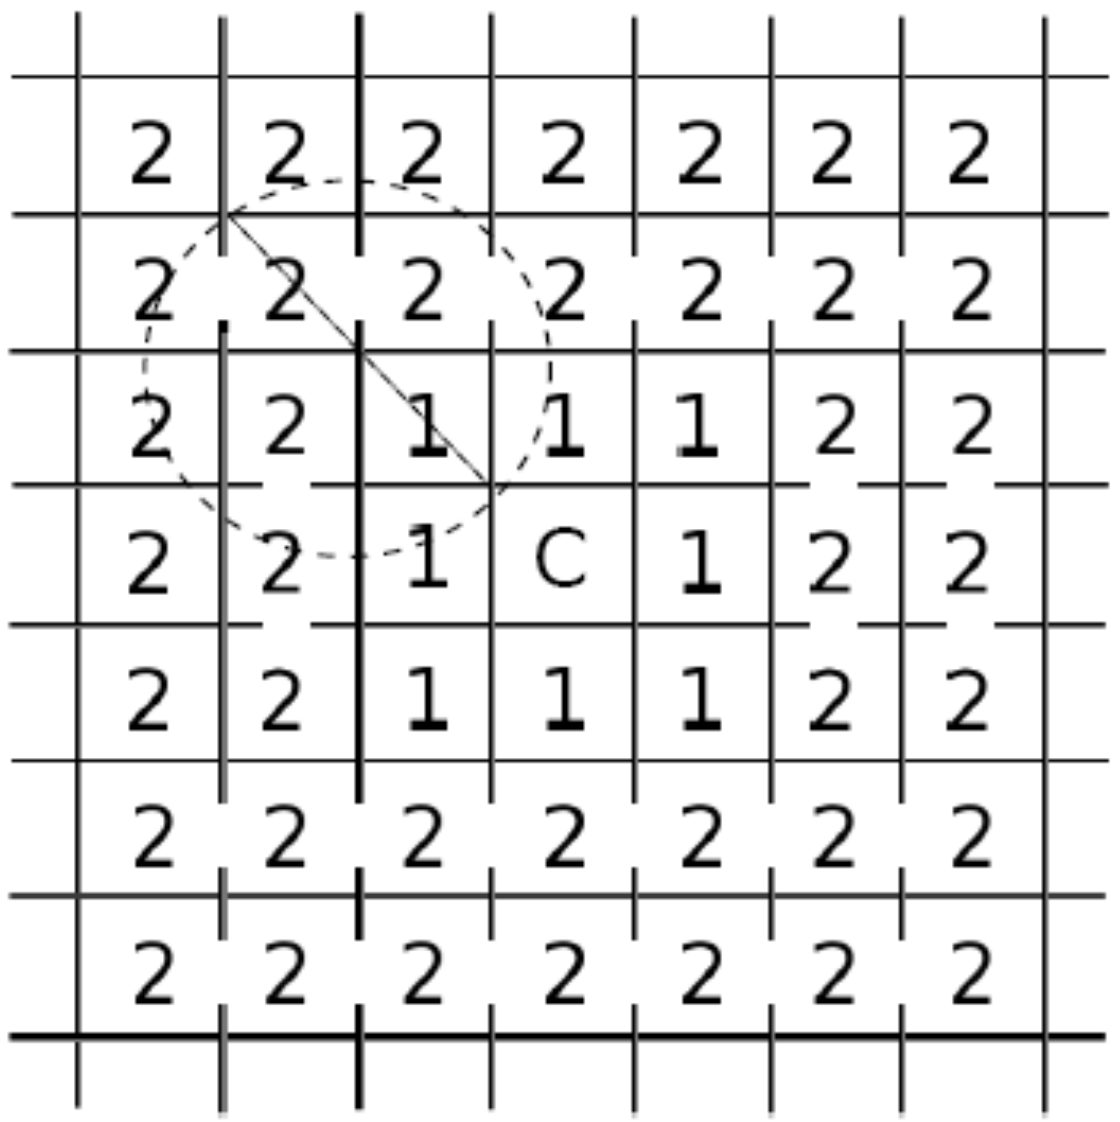
\includegraphics[width=0.25\textwidth]{img/grid8.png}};
\end{frame}


\begin{frame}{Distance-Based Outlier Detection: A Grid-Based Method II}
	\textcolor{faugray}{\textbf{Cell Pruning Rules}}
	\begin{itemize}
		\item Total number of objects in cell $\mathbf{C}$: $a$.
		\item Total number of objects in level-1 cells: $b_1$.
		\item Total number of objects in level-2 cells: $b_2$.
	\end{itemize}
	\begin{itemize}
		\item \textbf{Level-1 cell pruning rule}:
		      \begin{itemize}
			      \item If $a + b_1 > \lceil \pi n \rceil$, then every object $\mathbf{o}$ in $\mathbf{C}$ is not a $\mathbf{DB}(r, \pi)$-outlier, because all objects in $\mathbf{C}$ and the level-1 cells are in the $r$-neighborhood of $\mathbf{o}$, and there are at least $\lceil \pi n \rceil$ such objects.
		      \end{itemize}
		\item \textbf{Level-2 cell pruning rule:}
		      \begin{itemize}
			      \item If $a + b_1 + b_2 < \lceil \pi n \rceil + 1$, then all objects in $\mathbf{C}$ are $\mathbf{DB}(r, \pi)$-outliers, because all of their $r$-neighborhoods have less than $\lceil \pi n \rceil$ other objects.
		      \end{itemize}
		\item \textbf{Only need to check the objects that cannot be pruned.}
		      \begin{itemize}
			      \item Even for such an object $\mathbf{o}$, \\
			            only need to compute the distance between $\mathbf{o}$ and the objects in level-2 cells.
			            \begin{itemize}
				            \item Since beyond level-2, distance from $\mathbf{o}$ is more than $r$.
			            \end{itemize}
		      \end{itemize}
	\end{itemize}
\end{frame}


\begin{frame}{Density-Based Outlier Detection}
	\begin{itemize}
		\item Density around \textbf{outlier} object \textbf{significantly different}
		\item Methods use a \textit{relative density} of an object against is neighbor.
		\item This indicates to which degree an object is considered an outlier.
		\item \textbf{\color{airforceblue}Local outliers:} Outliers compared to their local neighborhoods, not to global data distribution.
	\end{itemize}
	\vspace*{1em}
	\textbf{Figure on the right:}
	\begin{itemize}
		\item Objects $\textbf{o}_1$ and $\textbf{o}_2$ are local outliers to $C_1$, $\textbf{o}_3$ is a global outlier, \\
		      but $\textbf{o}_4$ is not an outlier.
		\item However, distance of $\textbf{o}_1$ and $\textbf{o}_2$ to objects in dense cluster $C_1$ \\
		      is smaller than average distance in sparse cluster $C_2$.
		\item Hence, $\textbf{o}_1$ and $\textbf{o}_2$ are not distance-based outliers.
	\end{itemize}
	\tikzoverlay at (10cm,3cm) {
		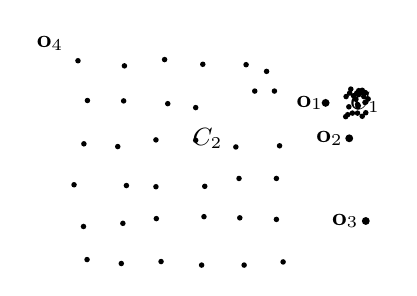
\begin{tikzpicture}[thick,scale=0.5, every node/.style={scale=5}]
			\fill (0.14, 0.02)  circle (0.7mm) (0.05, 0.86)  circle (0.7mm) (-0.19, 1.92)  circle (0.7mm) (0.06, 2.96)  circle (0.7mm) (0.15, 4.06)  circle (0.7mm) (-0.09, 5.07)  circle (0.7mm) (1.01, -0.08)  circle (0.7mm) (1.05, 0.94)  circle (0.7mm) (1.14, 1.9)  circle (0.7mm) (0.92, 2.89)  circle (0.7mm) (1.07, 4.05)  circle (0.7mm) (1.09, 4.94)  circle (0.7mm) (2.02, -0.03)  circle (0.7mm) (1.9, 1.06)  circle (0.7mm) (1.89, 1.87)  circle (0.7mm) (1.89, 3.06)  circle (0.7mm) (2.19, 3.98)  circle (0.7mm) (2.11, 5.1)  circle (0.7mm) (3.05, -0.12)  circle (0.7mm) (3.11, 1.11)  circle (0.7mm) (3.13, 1.88)  circle (0.7mm) (2.9, 3.05)  circle (0.7mm) (2.9, 3.88)  circle (0.7mm) (3.08, 4.98)  circle (0.7mm) (4.13, -0.12)  circle (0.7mm) (4.02, 1.08)  circle (0.7mm) (4.0, 2.08)  circle (0.7mm) (3.92, 2.88)  circle (0.7mm) (4.4, 4.3)  circle (0.7mm) (4.18, 4.97)  circle (0.7mm) (5.12, -0.04)  circle (0.7mm) (4.95, 1.04)  circle (0.7mm) (4.95, 2.08)  circle (0.7mm) (5.03, 2.91)  circle (0.7mm) (4.9, 4.3)  circle (0.7mm) (4.7, 4.8)  circle (0.7mm);

			% cluster
			\fill (7.22, 4.02)  circle (0.7mm) (7.01, 3.74)  circle (0.7mm) (7.17, 4.16)  circle (0.7mm) (7.04, 4.31)  circle (0.7mm) (7.28, 4.1)  circle (0.7mm) (7.22, 3.75)  circle (0.7mm) (6.99, 4.25)  circle (0.7mm) (7.13, 3.66)  circle (0.7mm) (7.03, 3.93)  circle (0.7mm) (6.84, 4.35)  circle (0.7mm) (6.72, 4.16)  circle (0.7mm) (7.14, 4.27)  circle (0.7mm) (6.88, 3.74)  circle (0.7mm) (7.04, 4.21)  circle (0.7mm) (6.79, 3.9)  circle (0.7mm) (7.01, 3.96)  circle (0.7mm) (7.13, 4.32)  circle (0.7mm) (6.71, 3.65)  circle (0.7mm) (6.76, 3.7)  circle (0.7mm) (7.21, 4.26)  circle (0.7mm) (7.02, 3.9)  circle (0.7mm) (7.2, 4.01)  circle (0.7mm) (6.91, 4.18)  circle (0.7mm) (6.81, 4.25)  circle (0.7mm) (6.97, 4.09)  circle (0.7mm);

			% outlier O3
			\fill (7.22, 1)  circle (1mm);
			\node[scale = 0.2] at (6.7, 1) {\small $\textbf{o}_3$};

			% O1
			\fill (6.2, 4)  circle (1mm);
			\node[scale = 0.2] at (5.8, 4) {\small $\textbf{o}_1$};

			% O2
			\fill (6.8, 3.1)  circle (1mm);
			\node[scale = 0.2] at (6.3, 3.1) {\small $\textbf{o}_2$};
			\node[scale = 0.2] at (7.2, 4) {\small $C_1$};
			\node[scale = 0.2] at (3.2, 3.1) {\small $C_2$};
			\node[scale = 0.2] at (-0.8, 5.5) {\small $\textbf{o}_4$};
		\end{tikzpicture}};
\end{frame}


\begin{frame}{Density-Based Outlier Detection: Measure Relative Density}
	\begin{itemize}
		\item Use the \textbf{relative density} of an object against its neighbors \\
		      as the indicator of the degree of the object being an outlier.
		\item \textbf{{\color{airforceblue}$k$-distance} of an object $\mathbf{o}$:} $d_k(\mathbf{o})$.

		      Distance between $\mathbf{o}$ and its $k$-nearest neighbors.
		\item Distance $d(\mathbf{o}, \mathbf{p})$ between $\mathbf{o}$ and its $k$-nearest neighbour $p$.
		      \begin{itemize}
			      \item At least $k$-objects $\textbf{o}' \in \mathbf{D} - \{\mathbf{o}\}$
			            such that $d(\mathbf{o}, \mathbf{o}') \leq d(\mathbf{o}, \mathbf{p})$.
			      \item At most $k-1$ objects $\mathbf{o}'' \in \mathbf{D} - \{\mathbf{o}\}$
			            such that $d(\mathbf{o}, \mathbf{o}'') > d(\mathbf{o}, \mathbf{p})$.
		      \end{itemize}
		\item $k$-distance neighborhood of $\mathbf{o}$:
		      \begin{itemize}
			      \item $N_k(\mathbf{o}) = \{\mathbf{o}' \; \vert \; \mathbf{o}' \in \mathbf{D}, d(\mathbf{o}, \mathbf{o}') \leq d_k(\mathbf{o})\}$.
			      \item $N_k(\mathbf{o})$ could be bigger than $k$ \\
			            since multiple objects may have identical distance to $\mathbf{o}$.
		      \end{itemize}
		\item Measure local distance by using the \textit{average distance} from objects in $N_k(\mathbf{o})$.
		\item \textbf{Problem:} If $\mathbf{o}$ has very close neighbors $\mathbf{o}'$, statistical fluctuations of the distance measure can be undesirable high. Overcome this problem with a \underline{reachability distance}.
	\end{itemize}
\end{frame}


\begin{frame}{Density-Based Outlier Detection: Reachability Distance}
	\begin{itemize}
		\item \textbf{\color{airforceblue}Reachability distance from $\mathbf{o'}$ to $\mathbf{o}$:}
		      \begin{align*}
			      \text{reachdist}_k(\mathbf{o}' \leftarrow \mathbf{o}) = \max \{d_k(\mathbf{o}), d(\mathbf{o},\mathbf{o}')\},
		      \end{align*}

		      where $k$ is a user-specified parameter that adds a smoothing effect.
		\item $k$ specifies the minimum neighborhood to be examined to determine the local density of an object.
		\item \textbf{Reachability distance is not symmetric!}
		      \begin{align*}
			      \text{reachdist}_k(\mathbf{o}' \leftarrow \mathbf{o}) \neq \text{reachdist}_k(\mathbf{o} \leftarrow \mathbf{o}')
		      \end{align*}
		\item \textbf{Local reachability density of $\mathbf{o}$:}
		      \begin{align*}
			      \text{ldr}_k(\mathbf{o}) = \frac{||N_k(\mathbf{o})||}{\sum_{\mathbf{o'} \in N_k(\mathbf{o})} \text{reachdist}_k(\mathbf{o'} \leftarrow \mathbf{o})}.
		      \end{align*}
	\end{itemize}
\end{frame}


\begin{frame}{Density-Based Outlier Detection: Local Outlier Factor (LOF)}
	\begin{itemize}
		\item LOF is the average of the ratio of the local reachability density of $\mathbf{o}$ and \\
		      those of $\mathbf{o}$'s $k$-nearest neighbors.
		\item The lower $\text{ldr}$ and the higher $\text{ldr}$ of the $k$-nearest neighbors of $\mathbf{o}$,\\
		      then the higher the LOF value.
		\item LOF of $\mathbf{o}$ is defined as:
		      \begin{align*}
			      \text{LOF}_k(\mathbf{o}) = \frac{\sum_{\mathbf{o'} \in N_k(\mathbf{o})} \frac{\text{lrd}_k(\mathbf{o'})}{\text{lrd}_k(\mathbf{o})}}{||N_k(\mathbf{o})||} =
			      \sum_{\mathbf{o'} \in N_k(\mathbf{o})} \text{lrd}_k(\mathbf{o'}) \cdot \sum_{\mathbf{o'} \in N_k(\mathbf{o})} \text{reachdist}_k(\mathbf{o'} \leftarrow \mathbf{o}).
		      \end{align*}
		\item This captures a local outlier whose local density is relatively low comparing to the local densities of its $k$-NN.

	\end{itemize}

\end{frame}
